% Dokumentklassen sættes til memoir.
% Manual: http://ctan.org/tex-archive/macros/latex/contrib/memoir/memman.pdf
\documentclass[a4paper,10pt]{article}
\usepackage[a4paper]{geometry}
% Danske udtryk (fx figur og tabel) samt dansk orddeling og fonte med

% danske tegn. Hvis LaTeX brokker sig over æ, ø og å skal du udskifte
% "utf8" med "latin1" eller "applemac". 
\usepackage[utf8]{inputenc}
\usepackage[danish]{babel}
\usepackage[T1]{fontenc}
 
\usepackage{cite}
\usepackage{natbib}
% Matematisk udtryk, fede symboler, theoremer og fancy ting (fx kædebrøker)
\usepackage{amsmath,amssymb}
\usepackage{bm}
\usepackage{amsthm}
\usepackage{tikz}
%\usepackage{mathtools}
% Kodelisting. Husk at læse manualen hvis du vil lave fancy ting.
% Manual: http://mirror.ctan.org/macros/latex/contrib/listings/listings.pdf
\usepackage{listings}
\usepackage{verbatim}
 
% Fancy ting med enheder og datatabeller. Læs manualen til pakken
% Manual: http://www.ctan.org/tex-archive/macros/latex/contrib/siunitx/siunitx.pdf
%\usepackage{siunitx}
% Indsættelse af grafik.
\usepackage{graphicx}
%\usepackage{bussproofs}

% Reaktionsskemaer. Læs manualen for at se eksempler.
% Manual: http://www.ctan.org/tex-archive/macros/latex/contrib/mhchem/mhchem.pdf
%\usepackage[version=3]{mhchem}
\author{Lau Skorstengaard, 20103173 \\Christian Budde Christensen, 20103616}
\title{Serverbaseret Webprogrammering\\4. Aflevering}

\begin{document}
\maketitle
\section*{Opgave 3}
Den originale \texttt{GuessingGame.xact} gemte og beregnede XHTML i \texttt{UserState} objektet. Denne ville også indeholde alle \texttt{SubmitHandler} objekter, som direkte ændrede i XHTML outputtet og sendte det til klienten ved hjælp af \texttt{update} metoden. Spillet havde kun tre metoder \texttt{start}, \texttt{play} og \texttt{record}, \texttt{start} sørgede for at starte spillet og initalizere brugerens ``session'', \texttt{record} viste hvem der havde hiscoren og \texttt{play} stod for at vise spillet. Som sagt havde session-objektet al ansvar for at vise spillet. Hver gang en form blev submitted, ville handleren enten tilføje en besked til en form-template eller rydde indholdet og tilføje noget nyt. Dette afspejlede ikke control-flowet særlig godt og førte hurtigt til flere nested if's. 
\section*{Opgave 4}
\begin{center}
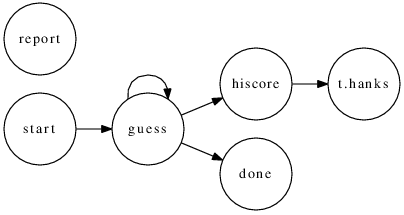
\includegraphics[width=10cm]{graphs/g0.png}
\end{center}
Controlflowet er afbilledet i ovenstående graf. Ud fra denne har vi lavet metoderne \texttt{guess},  \texttt{done},  \texttt{hiscore} og  \texttt{thanks}. Der navigeres mellem disse metoder via submit handlers, som returnerer en URL afhængig af brugerens handlinger. Der er dessuden tilføjet et filter, som sørger for at ingen ufortjent sætter sig selv på highscoren.  
\section*{Opgave 5}
Den største forskel mellem JWIG og Struts/JSF er fokus på XML's korrekthed, dette medfører flere garantier for sidens korrekthed, og dermed større modstandskraft mod eksempelvis XSS angreb. Derudover kræver frameworket minimal konfiguration og kedelige, trivielle opgaver, som form submit er abstraheret væk for udvikleren. JWIG har både komponenter af action-baserede framworks, som Struts, og component-baserede frameworks, som JSF.  

\end{document}
